% main.tex -- AI-Directed Prediction of Thermoelastic Wave Propagation
%             in Geological Media. Diploma defence deck, IITU 2026.
% Theme: UU beamer (kept from upstream skeleton).

\documentclass[aspectratio=169,10pt]{beamer}
\usetheme[showlogo,nosectionpage]{UU}

\usepackage{booktabs}
\usepackage{array}

% -- Metadata -----------------------------------
\title[AI-Directed Thermoelastic Prediction]{%
  AI-Directed Prediction of Thermoelastic Wave Propagation%
  \texorpdfstring{\\}{ }%
  in Geological Media%
}
\subtitle{A 2D physics-aware surrogate modelling framework}

\author[Group of 4]{%
  Kasymkhanov Timur \and
  Askarov Insar \and
  Kaidrakhmetova Dinara \and
  Nurshanov Dias%
}
\addinstitute{1}{International Information Technology University, Almaty}
\multiauthor
\venue{Bachelor's diploma defence, 2026}
\institute{International Information Technology University}
\date{\today}

\begin{document}

% ===========================================
%  TITLE
% ===========================================

\begin{frame}[plain]
  \titlepage
  \vfill
  \begin{center}\footnotesize
    Research adviser: \textbf{Bakhyt N. Alipova} (PhD, Applied Mathematics)
  \end{center}
\end{frame}

% Reset to single-author for the rest of the deck.
\subtitle{}
\clearinstitutes
\singleauthor

% ===========================================
%  TABLE OF CONTENTS
% ===========================================
\begin{frame}{Outline}
  \tableofcontents
\end{frame}

% ===========================================
\section{Motivation and Problem}
% ===========================================

\begin{frame}{Research Motivation}
  \begin{block}{Why AI surrogates for thermoelastic geological simulations}
    \begin{enumerate}
      \item \textbf{Full simulations are expensive.}
            Coupled transient thermoelastic simulations require fine spatial
            resolution and repeated parameter sweeps.
      \item \textbf{AI surrogates reduce repeated cost.}
            A trained model approximates field evolution orders of magnitude
            faster than running the numerical solver each time.
      \item \textbf{Physics remains the reference.}
            The goal is not to replace physics, but to use it for problem
            formulation, validation, and interpretation.
    \end{enumerate}
  \end{block}
\end{frame}

\begin{frame}{Core Research Question}
  \begin{exampleblock}{Question}
    Can neural surrogate models reproduce the main physical patterns of
    \emph{thermoelastic wave propagation in 2D plane-strain geological media}?
  \end{exampleblock}
  \vskip 4pt
  \begin{columns}[T]
    \begin{column}{0.24\textwidth}
      \begin{block}{\small 1.\ Input}
        Geometry\\Material params\\Source conditions
      \end{block}
    \end{column}
    \begin{column}{0.24\textwidth}
      \begin{block}{\small 2.\ Physics}
        Heat conduction\\Thermal expansion\\Elastic motion
      \end{block}
    \end{column}
    \begin{column}{0.24\textwidth}
      \begin{block}{\small 3.\ Surrogate}
        PINN\\FNO\\MeshGraphNet\\Transformer
      \end{block}
    \end{column}
    \begin{column}{0.24\textwidth}
      \begin{block}{\small 4.\ Output}
        Temperature $T$\\Displacement $(u,v)$\\Directional response
      \end{block}
    \end{column}
  \end{columns}
\end{frame}

\begin{frame}{Physical Scenario}
  \begin{columns}[T]
    \begin{column}{0.55\textwidth}
      A planar geological domain
      $\Omega \subset \mathbb{R}^{2}$, fixed at
      $1\,\text{m}\times 1\,\text{m}$, exposed to a localised thermal
      source.
      \begin{itemize}
        \item \textbf{Domain.} 2D plane-strain rock cross-section.
        \item \textbf{Excitation.} Point thermal source at temperature
              $T_{\text{src}}=1500\,\text{K}$, reference state
              $T_{\text{ref}}=273.15\,\text{K}$.
        \item \textbf{Response.} Coupled temperature $T$ and in-plane
              displacement $(u,v)$ at a chosen probe.
        \item \textbf{Task.} Estimate the probe response without rerunning
              the full COMSOL solver.
      \end{itemize}
    \end{column}
    \begin{column}{0.42\textwidth}
      \begin{block}{Locked operating envelope}
        \footnotesize
        Source type \alert{point}, mechanical \alert{free},
        boundary \alert{prototype simplified}.
        Trained on 2D plane-strain only; cannot be pushed out of
        distribution from the client side.
      \end{block}
    \end{column}
  \end{columns}
\end{frame}

\begin{frame}{Thermoelastic Coupling Logic}
  \begin{enumerate}
    \item \textbf{Thermal excitation.}
          A local source changes the temperature field.
    \item \textbf{Thermal expansion.}
          Temperature change produces local material expansion.
    \item \textbf{Stress formation.}
          Constrained expansion creates stress gradients.
    \item \textbf{Elastic motion.}
          Stress gradients accelerate the displacement field.
    \item \textbf{Wave propagation.}
          The response travels through the geological medium.
  \end{enumerate}
  \vskip 6pt
  This chain is the same in classical thermoelasticity and in our
  surrogate models; the difference is only \emph{how} each stage is
  represented.
\end{frame}

% ===========================================
\sectionframe{Section 1 -- Classical Physical Theory}
\section{Classical Physical Theory}
% ===========================================

\begin{frame}{Heat Conduction with Mechanical Coupling}
  \begin{block}{Governing equation}
    \[
      k\,\nabla^{2}T - C\,\frac{\partial T}{\partial t}
      = \gamma\,T_{0}\,\frac{\partial \varepsilon_{kk}}{\partial t}
    \]
  \end{block}
  \footnotesize
  $T$ -- temperature field;\quad
  $k$ -- thermal conductivity;\quad
  $C$ -- volumetric heat capacity;\quad
  $\gamma$ -- thermoelastic coupling;\quad
  $T_{0}$ -- reference temperature;\quad
  $\varepsilon_{kk}$ -- volumetric strain.
  \vskip 4pt
  \normalsize
  Heat diffuses from the heated region toward colder zones, and
  mechanical deformation of the rock additionally drives temperature
  variation. This coupling is essential for modelling thermoelastic
  waves in geological media.
\end{frame}

\begin{frame}{Thermoelastic Stress--Strain Relation}
  \begin{block}{Constitutive law (Duhamel--Neumann)}
    \[
      \sigma_{ij} = \lambda\,\delta_{ij}\,\varepsilon_{kk}
      + 2\mu\,\varepsilon_{ij}
      - \gamma\,\delta_{ij}\,(T - T_{0})
    \]
  \end{block}
  \begin{columns}[T]
    \begin{column}{0.33\textwidth}
      \footnotesize
      \textbf{Stress tensor.}
      Internal forces produced inside the material under deformation
      or heating.
    \end{column}
    \begin{column}{0.33\textwidth}
      \footnotesize
      \textbf{Elastic part.}
      First two terms: linear elastic response from volumetric strain
      $\varepsilon_{kk}$ and shear $\varepsilon_{ij}$.
    \end{column}
    \begin{column}{0.33\textwidth}
      \footnotesize
      \textbf{Thermal part.}
      Last term: thermal expansion. Constrained expansion creates
      thermal stress.
    \end{column}
  \end{columns}
  \vskip 6pt
  \scriptsize
  $\sigma_{ij}$ stress, $\varepsilon_{ij}$ strain,
  $\delta_{ij}$ Kronecker, $\lambda,\mu$ Lam\'e parameters,
  $\gamma=3K\alpha$ coupling coefficient.
\end{frame}

\begin{frame}{Equation of Motion}
  \begin{block}{Dynamic balance in an elastic medium}
    \[
      \rho\,\frac{\partial^{2} u_{i}}{\partial t^{2}}
      = \frac{\partial \sigma_{ij}}{\partial x_{j}} + f_{i}
    \]
  \end{block}
  \vskip 4pt
  Substituting the Duhamel--Neumann stress relation connects
  $T$, $\varepsilon$, $\sigma$, and $(u,v)$ in a single coupled
  thermoelastic system.
  \vskip 8pt
  \[
    T \longrightarrow \Delta T \longrightarrow \varepsilon
    \longrightarrow \sigma \longrightarrow u
  \]
\end{frame}

\begin{frame}{Physical Fields and Variables}
  \footnotesize
  \begin{tabular}{@{}lll@{}}
    \toprule
    \textbf{Symbol} & \textbf{Meaning} & \textbf{Role} \\
    \midrule
    $T$               & Temperature                          & Thermal state of the medium \\
    $(u,v)$           & In-plane displacement                & Mechanical motion (2D) \\
    $\sigma_{ij}$     & Stress tensor                         & Internal force response \\
    $\varepsilon_{ij}$ & Strain tensor                       & Local deformation \\
    $\rho, C_{p}, k$  & Density, heat capacity, conductivity  & Thermal material properties \\
    $\alpha, \lambda, \mu$ & Expansion, Lam\'e parameters     & Thermoelastic material properties \\
    $\gamma$          & $3K\alpha$ coupling coefficient       & Thermomechanical coupling \\
    $Q, f$            & Heat source, body force               & Excitation terms \\
    \bottomrule
  \end{tabular}
  \vskip 8pt
  \normalsize
  All quantities live in a planar 2D plane-strain domain
  $\Omega \subset \mathbb{R}^{2}$ in the current prototype.
\end{frame}

% ===========================================
\section{Dataset and Surrogate Objective}
% ===========================================

\begin{frame}{Simulation Data}
  \begin{block}{COMSOL-derived ground truth}
    Numerical 2D plane-strain simulations provide the training set:
    geometry, mesh, material properties, and time-dependent thermal /
    displacement fields exported per node.
  \end{block}
  \vskip 4pt
  \begin{itemize}
    \item \textbf{Inputs.}
          Geometry, mesh, material properties (granite, sandstone,
          limestone, basalt), source position, observation time.
    \item \textbf{Outputs.}
          Temperature $T$, displacement components $(u,v)$,
          stress / strain diagnostics.
    \item \textbf{Pilot dataset.}
          Sandstone rod-in-collar experiment (4448 nodes, $\Delta t = 10^{-4}$\,s,
          101 time steps); extended to per-material 2D batches.
  \end{itemize}
\end{frame}

\begin{frame}{Surrogate Modelling Objective}
  Replace repeated COMSOL runs with a fast field prediction.
  \vskip 8pt
  \begin{enumerate}
    \item \textbf{Reference simulation.}
          COMSOL produces time-dependent physical fields under the
          locked thermoelastic operating envelope.
    \item \textbf{Model training.}
          Each surrogate learns from physical parameters and exported
          fields; PINN additionally enforces PDE residuals.
    \item \textbf{Fast inference.}
          New scenarios are evaluated through a unified REST contract
          without rerunning the full solver.
  \end{enumerate}
\end{frame}

% ===========================================
\sectionframe{Section 2 -- AI Models}
\section{AI Models}
% ===========================================

\begin{frame}{Physics-Informed Neural Network (PINN)}
  \begin{columns}[T]
    \begin{column}{0.55\textwidth}
      \begin{block}{Core idea}
        \begin{itemize}
          \item Point-wise MLP $f_{\theta}(x,y,t,\text{material})\to(T,u,v)$.
          \item Composite loss: supervised data MSE,
                velocity-consistency, elastic-wave residual,
                coupled heat-equation residual.
          \item Penalises physically inconsistent outputs even when
                data coverage is limited.
        \end{itemize}
      \end{block}
    \end{column}
    \begin{column}{0.42\textwidth}
      \begin{exampleblock}{Why it fits}
        \begin{itemize}
          \item Governing equations are known.
          \item Physical consistency is a key validation criterion.
          \item Works as the theory-aware baseline.
        \end{itemize}
      \end{exampleblock}
      \begin{alertblock}{Limit}
        \footnotesize
        Training is slow; residual weighting is delicate.
      \end{alertblock}
    \end{column}
  \end{columns}
\end{frame}

\begin{frame}{Fourier Neural Operator (FNO)}
  \begin{columns}[T]
    \begin{column}{0.55\textwidth}
      \begin{block}{Core idea}
        \begin{itemize}
          \item Operator-learning model for field-to-field prediction.
          \item Captures global spatial patterns through spectral
                convolutions.
          \item Efficient on structured-grid PDE data.
        \end{itemize}
      \end{block}
      \emph{Conceptual workflow:}
      input field
      $\to$ frequency-space patterns
      $\to$ learned operator
      $\to$ predicted field.
    \end{column}
    \begin{column}{0.42\textwidth}
      \begin{alertblock}{Current caveat}
        \footnotesize
        2D-adapted branch. Output normalisation is not yet calibrated:
        absolute temperature and displacement scales are outside the
        physical band. Direction sign also needs verification.
        \emph{Diagnostic branch, not a physical reference yet.}
      \end{alertblock}
    \end{column}
  \end{columns}
\end{frame}

\begin{frame}{MeshGraphNet}
  \begin{block}{Graph-based surrogate for irregular meshes}
    \begin{enumerate}
      \item \textbf{Geometry as a graph.}
            Mesh nodes become graph nodes; mesh connectivity becomes
            graph edges.
      \item \textbf{Local interaction.}
            Messages propagate information between neighbouring
            regions of the domain.
      \item \textbf{Fits geology.}
            Irregular rock geometry and heterogeneous media are
            naturally represented by graphs.
    \end{enumerate}
  \end{block}
  \begin{alertblock}{Limit}
    \footnotesize
    Current implementation is a fixed-horizon rollout; the requested
    observation time does not yet drive the number of message-passing
    steps. Absolute magnitudes inherit a 2D-dataset / 3D-checkpoint
    padding mismatch.
  \end{alertblock}
\end{frame}

\begin{frame}{Transformer-Based Neural Operator}
  \begin{columns}[T]
    \begin{column}{0.55\textwidth}
      \begin{block}{How it can be used}
        \begin{itemize}
          \item OFormer-style encoder--decoder with cross-attention.
          \item Tokens carry coordinates, current-state fields,
                and material properties.
          \item Predicts $(T,u,v)$ at queried coordinates.
        \end{itemize}
      \end{block}
    \end{column}
    \begin{column}{0.42\textwidth}
      \begin{exampleblock}{Strengths}
        \footnotesize
        Flexible coordinate-query model; the fastest route at
        inference time in the latency test.
      \end{exampleblock}
      \begin{alertblock}{Limit}
        \footnotesize
        Current loss is supervised MSE only; no physics-informed
        residuals yet. High memory demand for dense fields.
      \end{alertblock}
    \end{column}
  \end{columns}
\end{frame}

\begin{frame}{Qualitative Model Comparison}
  \footnotesize
  \begin{tabular}{@{}lccccc@{}}
    \toprule
    \textbf{Model} & \textbf{Physics} & \textbf{Accuracy} & \textbf{Speed} & \textbf{Generalisation} & \textbf{Interpretability} \\
    \midrule
    PINN          & High        & Medium--High         & Medium      & Medium                       & High \\
    FNO           & Medium      & Pending calibration  & High        & High on similar grids        & Medium \\
    MeshGraphNet  & Medium      & Medium--High         & Medium--High & High on irregular meshes    & Medium \\
    Transformer   & Low--Medium & High with data       & High        & Medium                       & Low--Medium \\
    \bottomrule
  \end{tabular}
  \vskip 8pt
  \normalsize
  Framing: PINN as the physics-consistency baseline,
  MeshGraphNet for mesh-aware prediction, Transformer for fast
  flexible queries, FNO once normalisation is corrected.
\end{frame}

% ===========================================
\sectionframe{Section 3 -- Implementation}
\section{Implementation}
% ===========================================

\begin{frame}{System Architecture}
  \begin{block}{Service-oriented prototype (docker-compose)}
    \footnotesize
    \begin{tabular}{@{}lll@{}}
      \toprule
      \textbf{Service} & \textbf{Port} & \textbf{Role} \\
      \midrule
      \texttt{frontend}            & 8080 & Vanilla HTML/CSS/JS single-page app, nginx \\
      \texttt{backend}             & 8000 & FastAPI orchestrator, unified v2 contract \\
      \texttt{pinn-service}        & 9003 & PINN MLP, supervised + physics residuals \\
      \texttt{fno-service}         & 9002 & FNO2d, supervised MSE \\
      \texttt{mgn-service}         & 9001 & MeshGraphNet rollout \\
      \texttt{transformer-service} & 9004 & OFormer-based autoregressive operator \\
      \bottomrule
    \end{tabular}
  \end{block}
  Each model service exposes the same prediction endpoint; the backend
  validates, resolves the geological medium from the catalogue, routes,
  and normalises the response.
\end{frame}

\begin{frame}{Unified Prediction Contract (v2)}
  \begin{block}{Request shape}
    \footnotesize
    Schema-versioned payload with $(x,y)$ source and probe inside the
    fixed $1\,\text{m}\times 1\,\text{m}$ unit square; observation time
    in seconds; locked scenario block (point thermal source, free
    mechanical constraint, prototype boundary).
  \end{block}
  \begin{block}{Response shape}
    \footnotesize
    Thermal $(T,\theta)$, in-plane displacement $(u,v)$ with magnitude,
    directional response (distance, azimuth, unit direction),
    temporal (travel time), model metadata, diagnostics.
  \end{block}
  \begin{exampleblock}{Locked invariants}
    \footnotesize
    $T_{\text{ref}}=273.15\,\text{K}$,
    $T_{\text{src}}=1500\,\text{K}$,
    domain $1\,\text{m}\times 1\,\text{m}$,
    no source frequency.
    Resolved server-side so clients cannot push trained models out of
    distribution.
  \end{exampleblock}
\end{frame}

\begin{frame}{Web Interface -- Landing}
  \begin{center}
    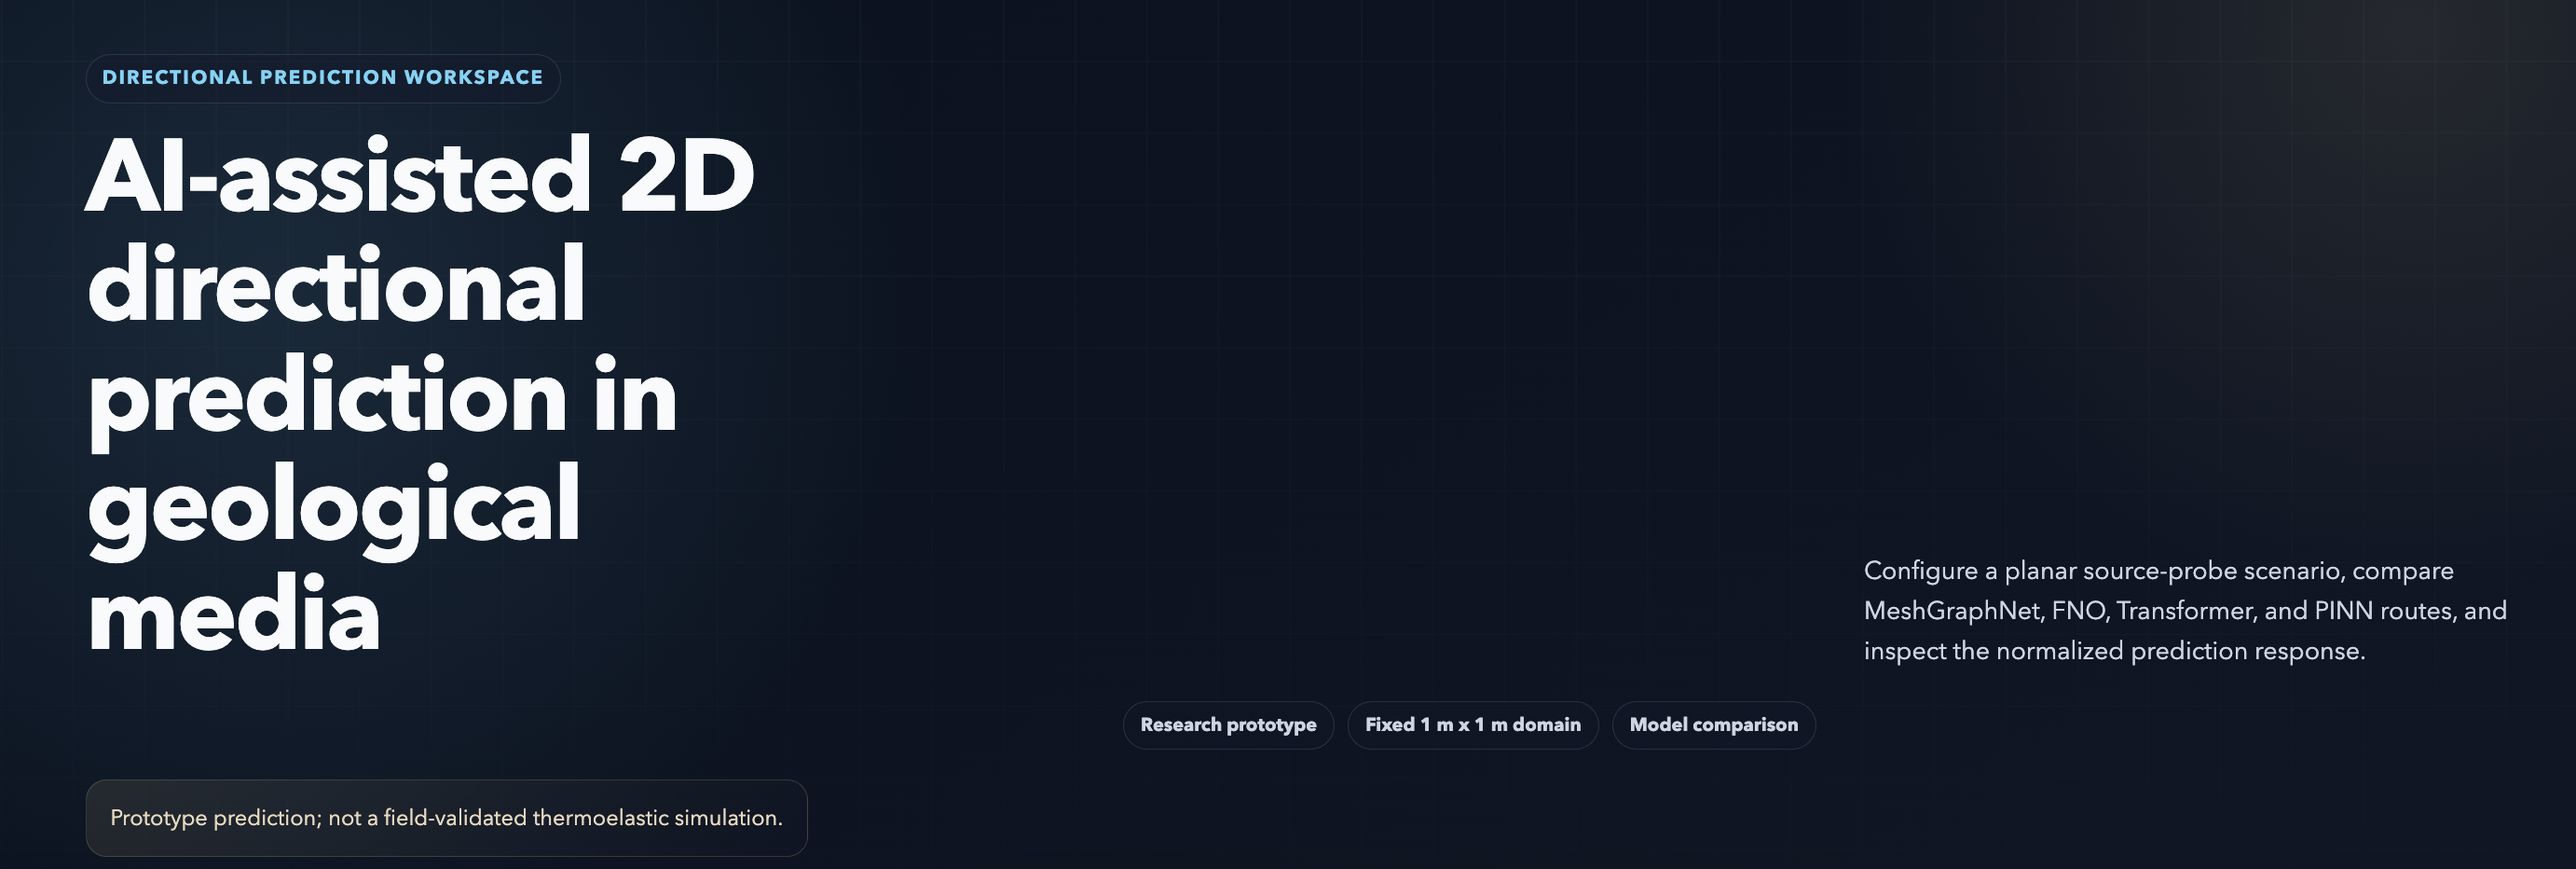
\includegraphics[width=0.95\textwidth]{img/web_title}
  \end{center}
  \vskip 4pt
  \footnotesize
  Static single-page application; no runtime framework. Three
  contextual chips pin the scope:
  \emph{research prototype}, \emph{fixed
  1\,m\,$\times$\,1\,m domain}, \emph{model comparison}. Every
  response carries a prototype-prediction disclaimer.
\end{frame}

\begin{frame}{Web Interface -- Planar Visualisation}
  \begin{columns}[T]
    \begin{column}{0.58\textwidth}
      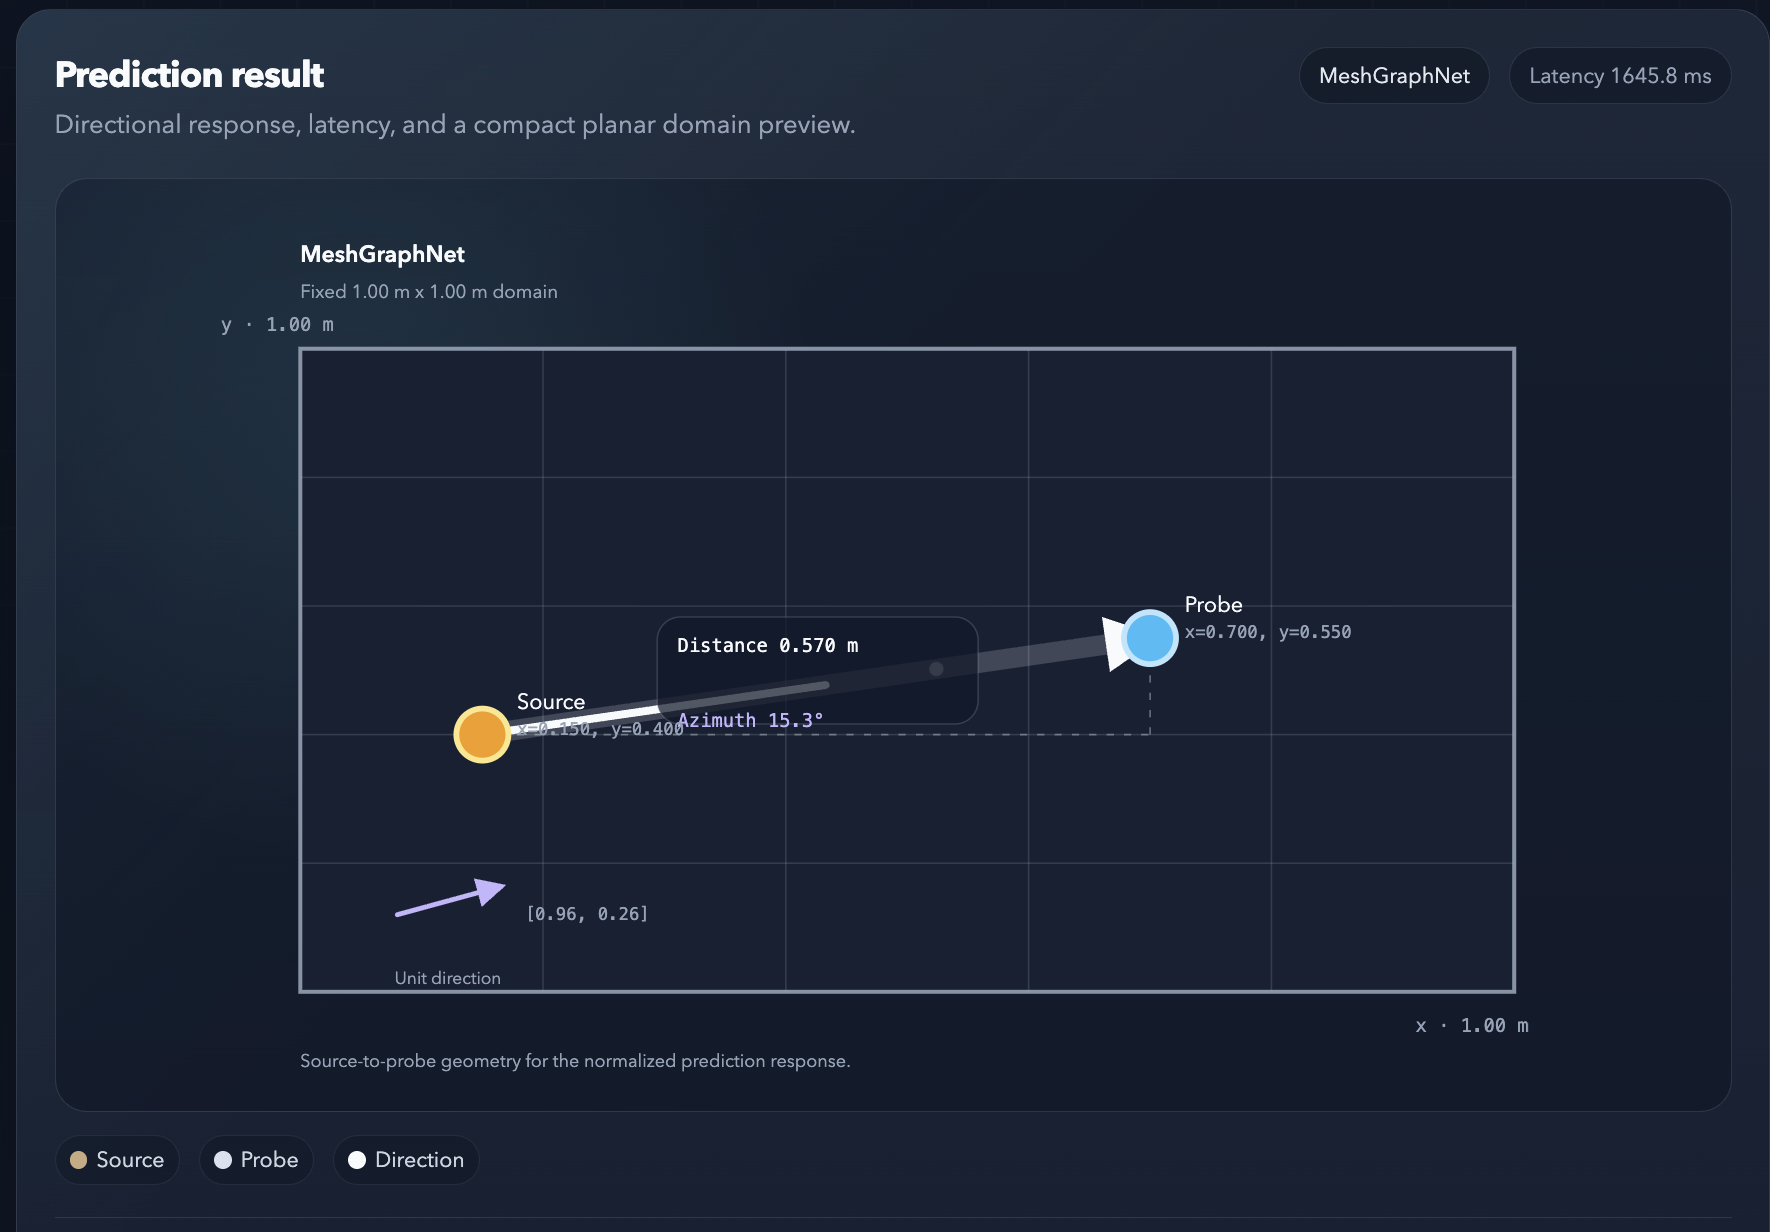
\includegraphics[width=\textwidth]{img/web_visualization}
    \end{column}
    \begin{column}{0.38\textwidth}
      \footnotesize
      \begin{itemize}
        \item Source (warm disc) and probe (cool disc) inside the unit
              square.
        \item Propagation arrow carries distance and azimuth.
        \item Unit-direction key in the bottom-left.
        \item Geometry computation is the same one the backend uses,
              so the SVG and numeric panels never disagree.
      \end{itemize}
    \end{column}
  \end{columns}
\end{frame}

\begin{frame}{Web Interface -- Prediction Result}
  \begin{columns}[T]
    \begin{column}{0.55\textwidth}
      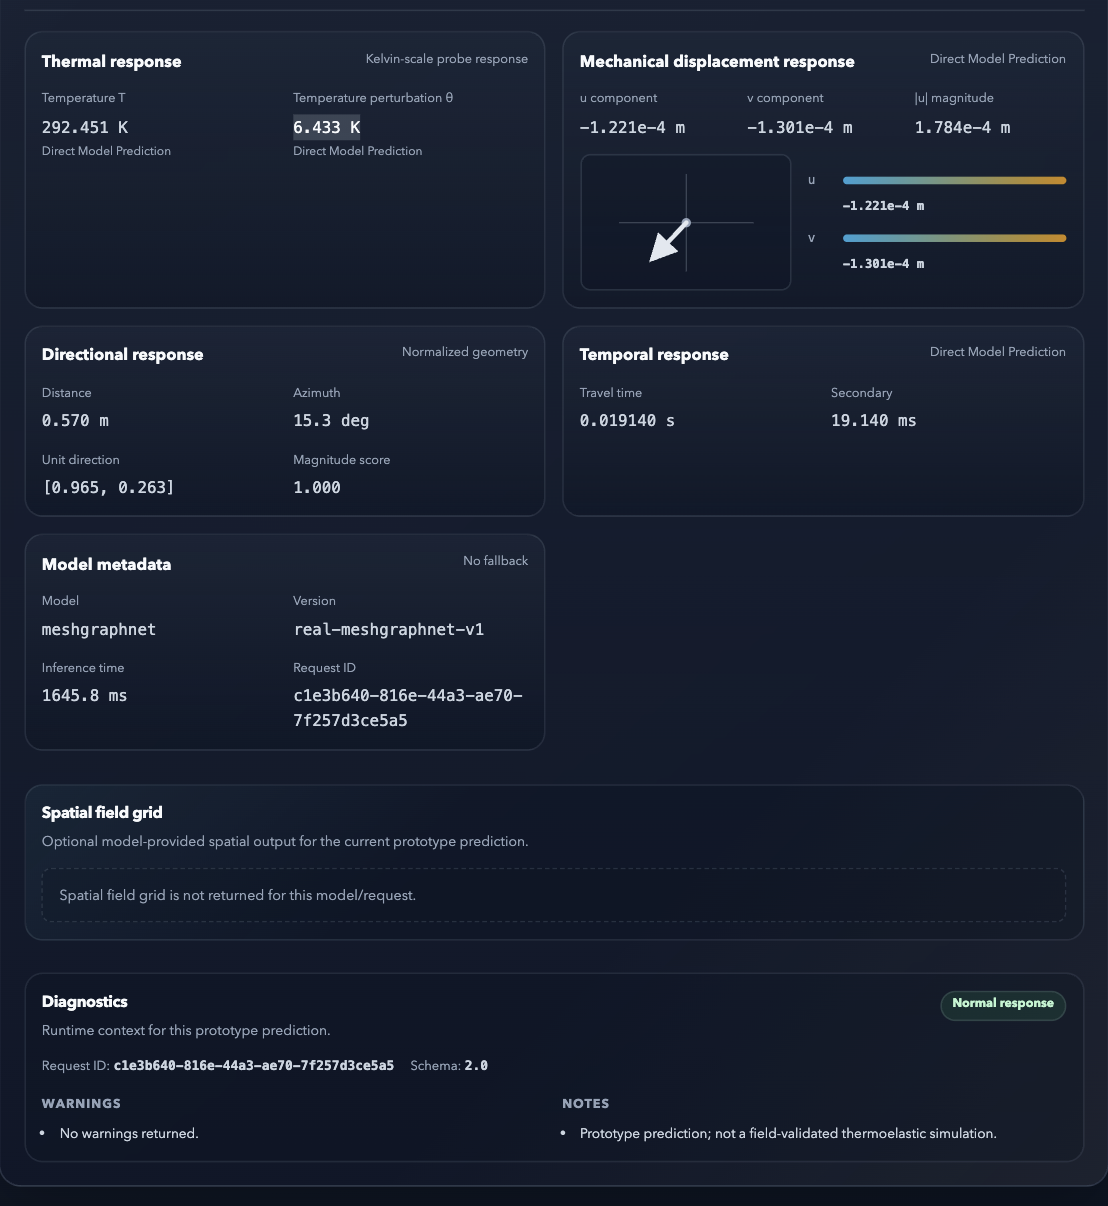
\includegraphics[width=\textwidth]{img/web_result}
    \end{column}
    \begin{column}{0.42\textwidth}
      \footnotesize
      Cards report the thermal response at the probe ($T$ and
      perturbation $\theta = T - T_{0}$), the in-plane displacement
      $(u,v)$ with magnitude, the directional response, the temporal
      response (travel time), and the model metadata. The diagnostics
      strip carries the run state, schema version, and any warnings
      returned by the backend.
    \end{column}
  \end{columns}
\end{frame}

% ===========================================
\sectionframe{Section 4 -- Experimental Results}
\section{Experimental Results}
% ===========================================

\begin{frame}{Experiment Status}
  \begin{block}{Evaluation setup}
    \begin{enumerate}
      \item \textbf{40 scenarios per material}, four materials
            (granite, sandstone, limestone, basalt).
      \item \textbf{$\mathbf{40\,\times\,4\,\times\,4 = 640}$ model
            responses} collected under the same v2 contract.
      \item \textbf{Zero fallback}: every plotted response is an active
            model output, not a mock.
      \item \textbf{2D plane-strain only} -- the operating envelope
            of all four trained surrogates.
    \end{enumerate}
  \end{block}
  \begin{alertblock}{FNO caveat}
    \footnotesize
    FNO is loaded, but its absolute temperature and displacement
    scales are outliers. Treated as a diagnostic branch in this
    comparison.
  \end{alertblock}
\end{frame}

\begin{frame}{Travel-Time Predictions}
  \begin{columns}[T]
    \begin{column}{0.55\textwidth}
      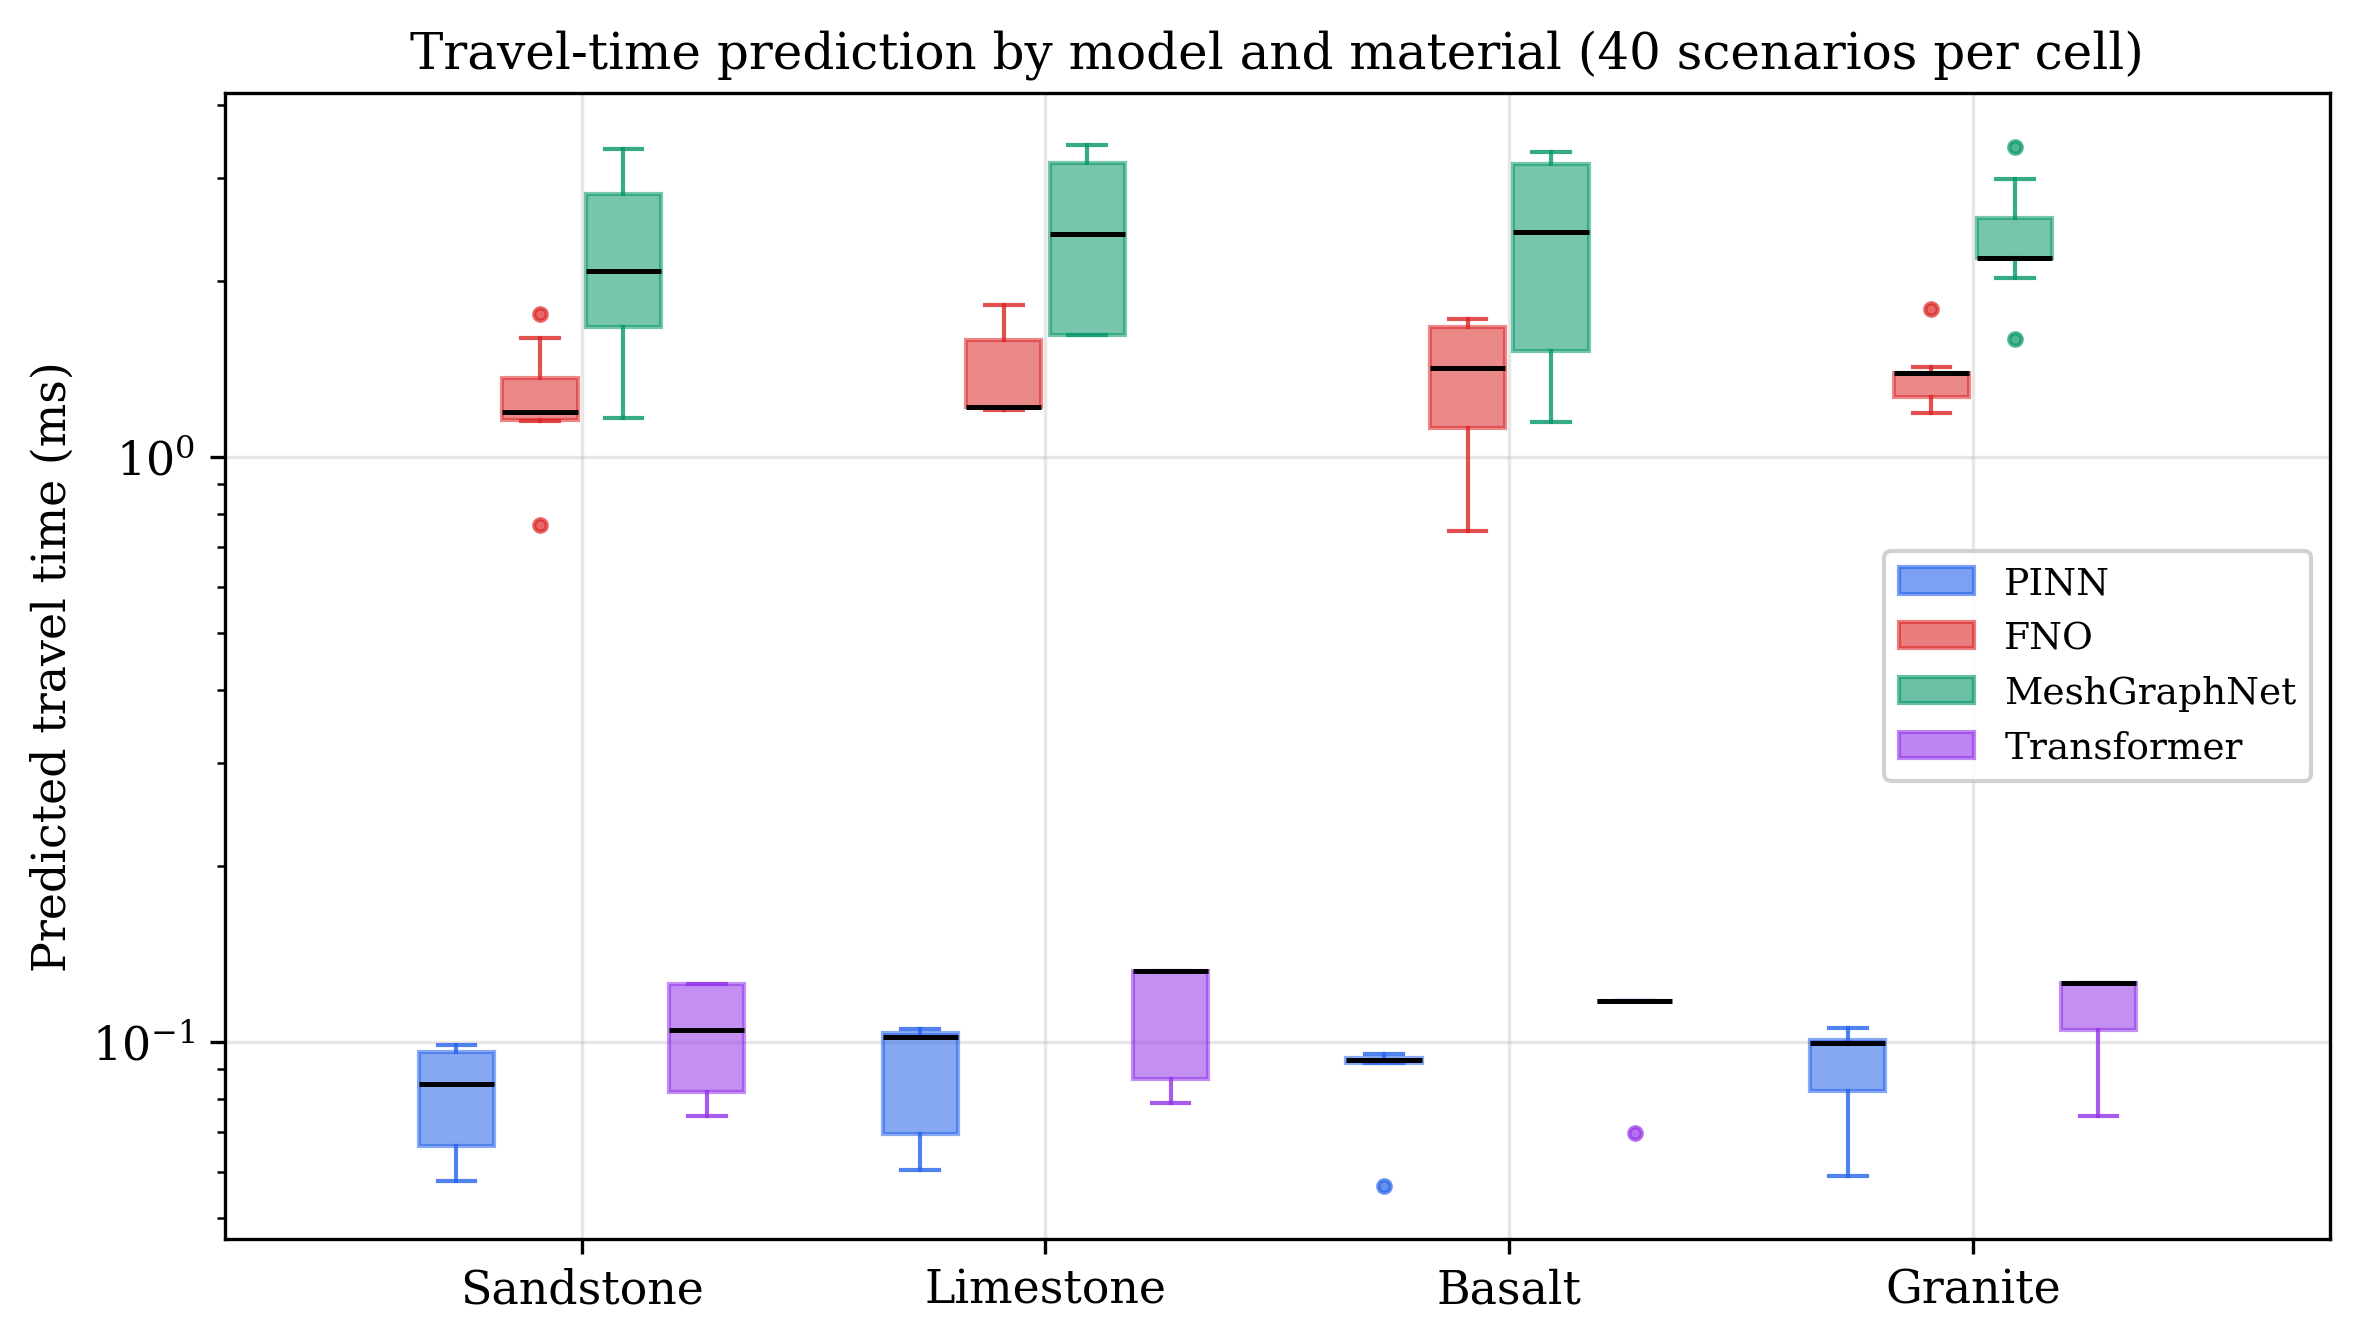
\includegraphics[width=\textwidth]{img/travel_time_by_model_material}
    \end{column}
    \begin{column}{0.42\textwidth}
      \footnotesize
      Mean travel time per route:
      \begin{itemize}
        \item PINN $\approx 0.11$\,ms
        \item Transformer $\approx 0.14$\,ms
        \item FNO $\approx 1.29$\,ms
        \item MeshGraphNet $\approx 2.47$\,ms
      \end{itemize}
      Sandstone is slightly slower than basalt for every route, which
      is consistent with its lower $V_{p}$. Model-family differences
      dominate the spread over material differences.
    \end{column}
  \end{columns}
\end{frame}

\begin{frame}{Accuracy Against Analytical Reference}
  \begin{columns}[T]
    \begin{column}{0.55\textwidth}
      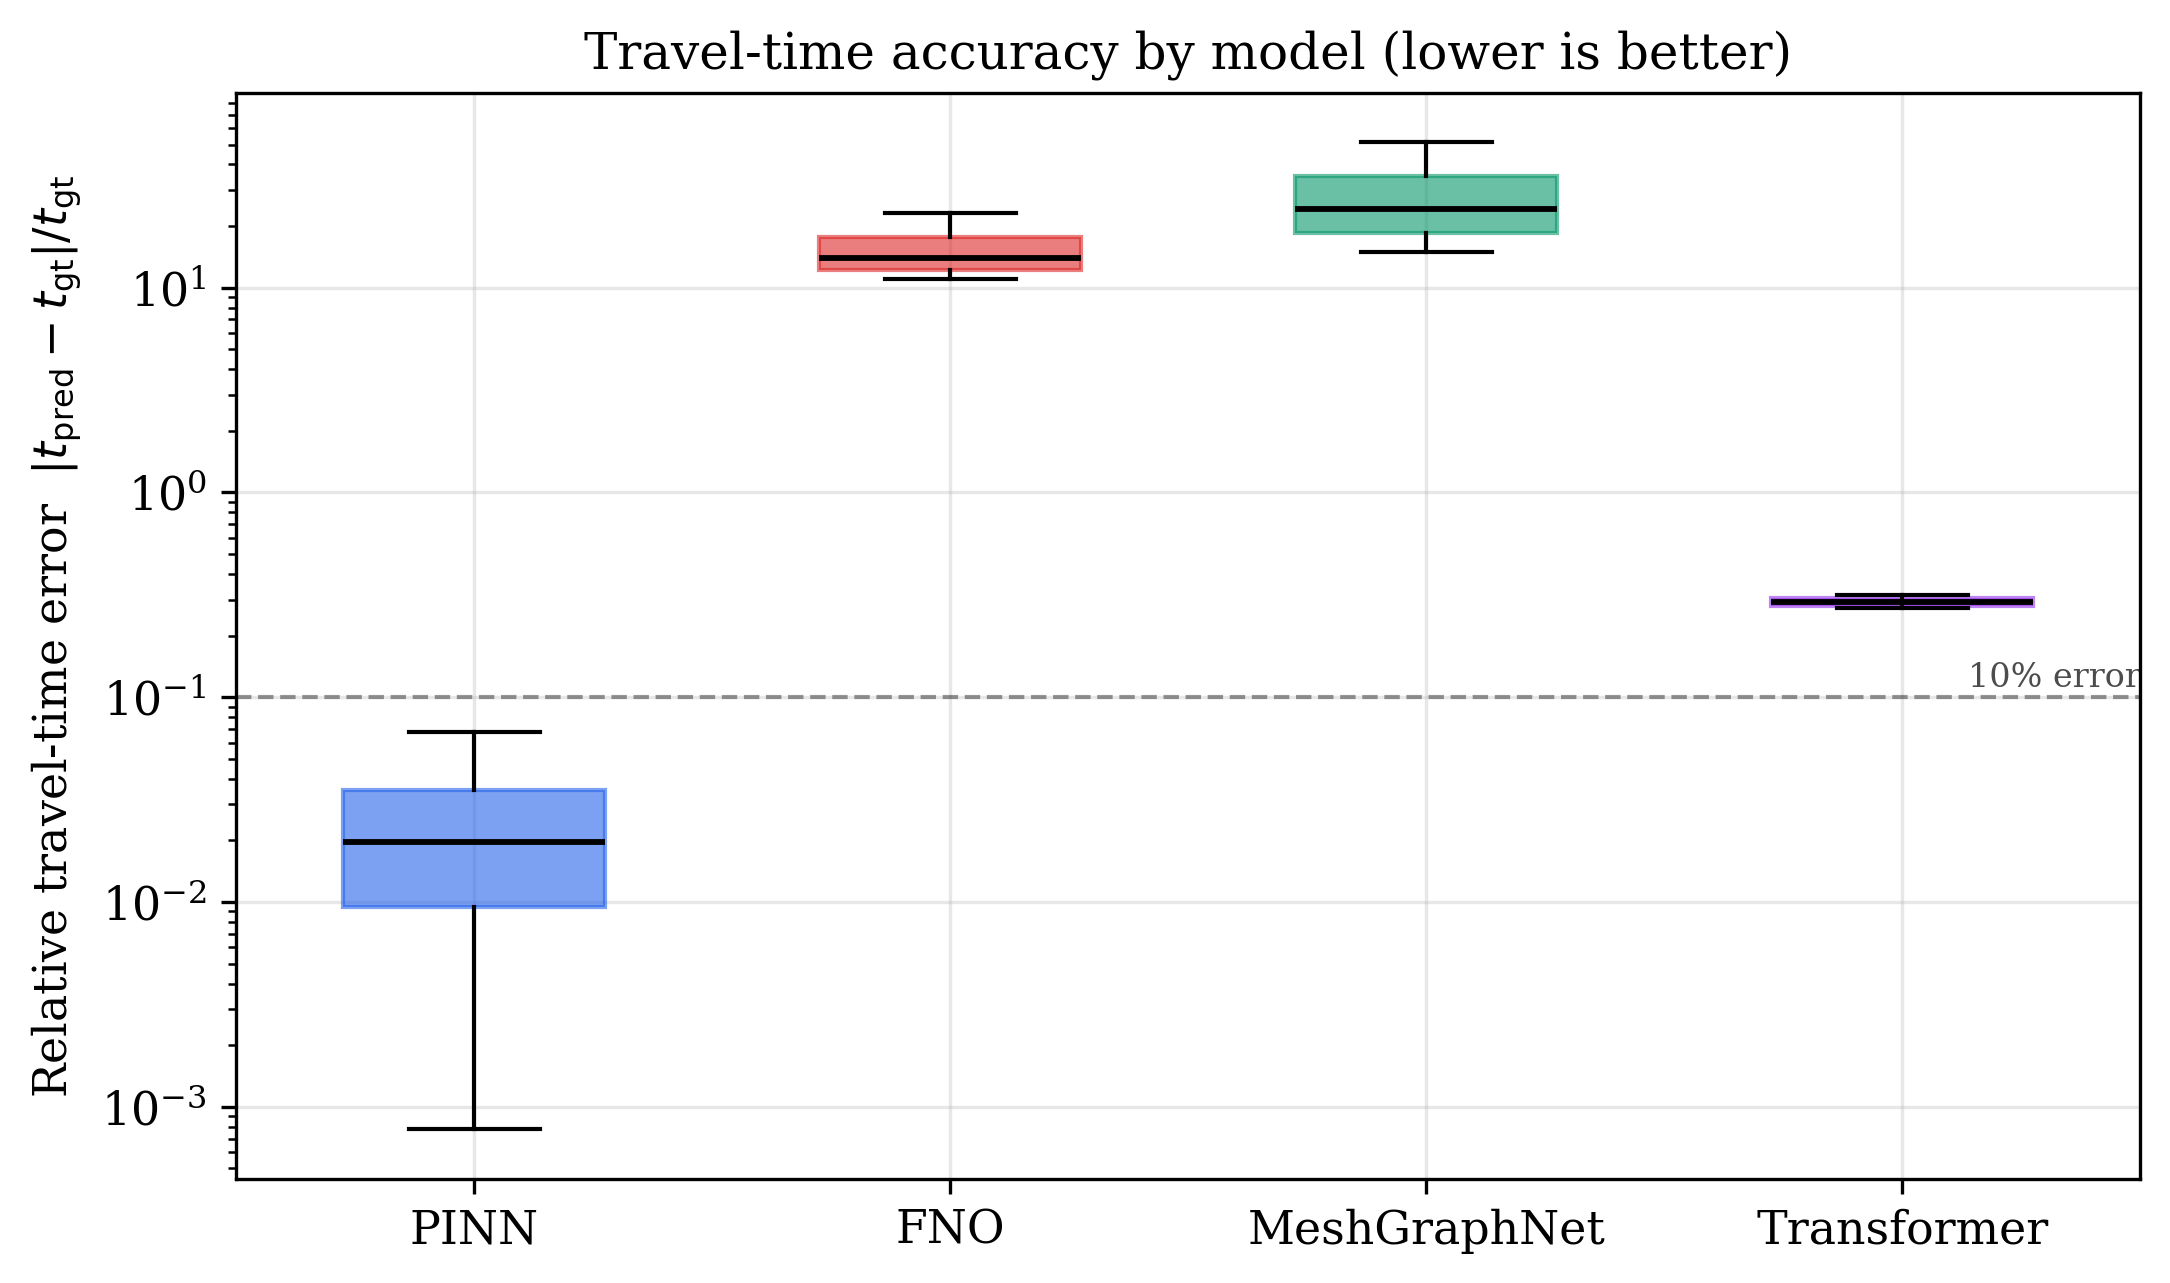
\includegraphics[width=\textwidth]{img/travel_time_relative_error}
    \end{column}
    \begin{column}{0.42\textwidth}
      \footnotesize
      Reference: analytical body-wave travel time $r / V_{p}$.
      \begin{tabular}{@{}lcc@{}}
        \toprule
        \textbf{Model} & \textbf{Median rel.\ error} & \textbf{Within 10\,\%} \\
        \midrule
        PINN         & $2.0\%$    & $100\%$ \\
        Transformer  & $29.2\%$   & $0\%$   \\
        FNO          & $1403.6\%$ & $0\%$   \\
        MGN          & $> 100\%$  & $0\%$   \\
        \bottomrule
      \end{tabular}
      \vskip 4pt
      PINN is the only route within the $10\%$ band on every scenario
      of the balanced sweep.
    \end{column}
  \end{columns}
\end{frame}

\begin{frame}{Inference Latency}
  \begin{columns}[T]
    \begin{column}{0.55\textwidth}
      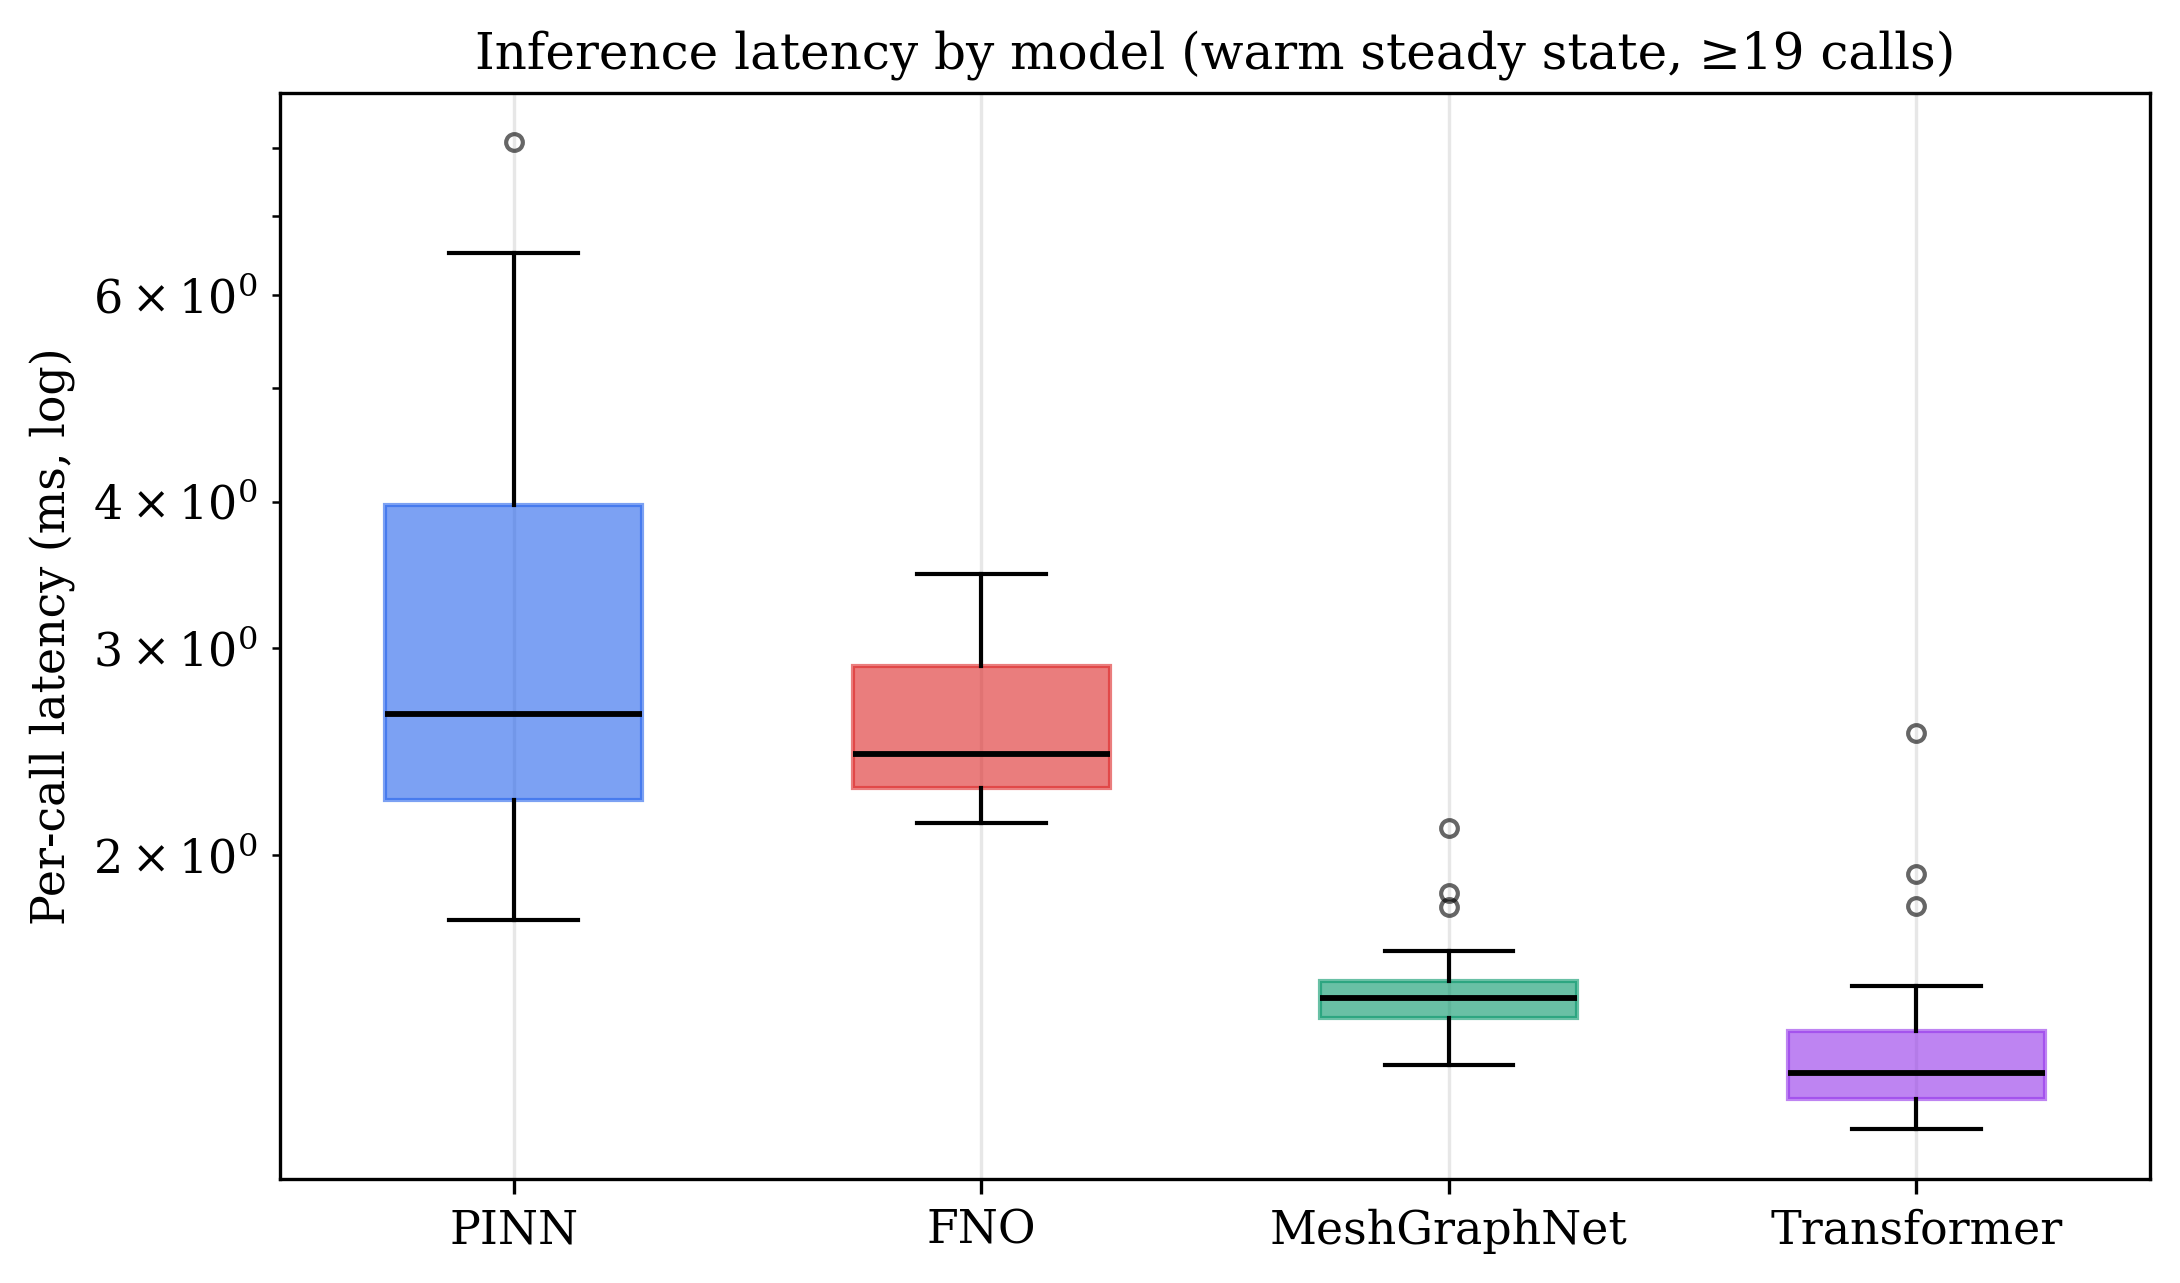
\includegraphics[width=\textwidth]{img/inference_latency_by_model}
    \end{column}
    \begin{column}{0.42\textwidth}
      \footnotesize
      All four routes return in under $10$\,ms on the development
      machine.
      \begin{itemize}
        \item Transformer $\approx 1.3$\,ms (median)
        \item MeshGraphNet $\approx 1.5$\,ms
        \item FNO $\approx 2.4$\,ms
        \item PINN $\approx 2.6$\,ms (longer upper tail)
      \end{itemize}
      Latency is reported as a prototype-level wall-clock measurement,
      not a production benchmark.
    \end{column}
  \end{columns}
\end{frame}

\begin{frame}{Time-Series Behaviour}
  \begin{columns}[T]
    \begin{column}{0.62\textwidth}
      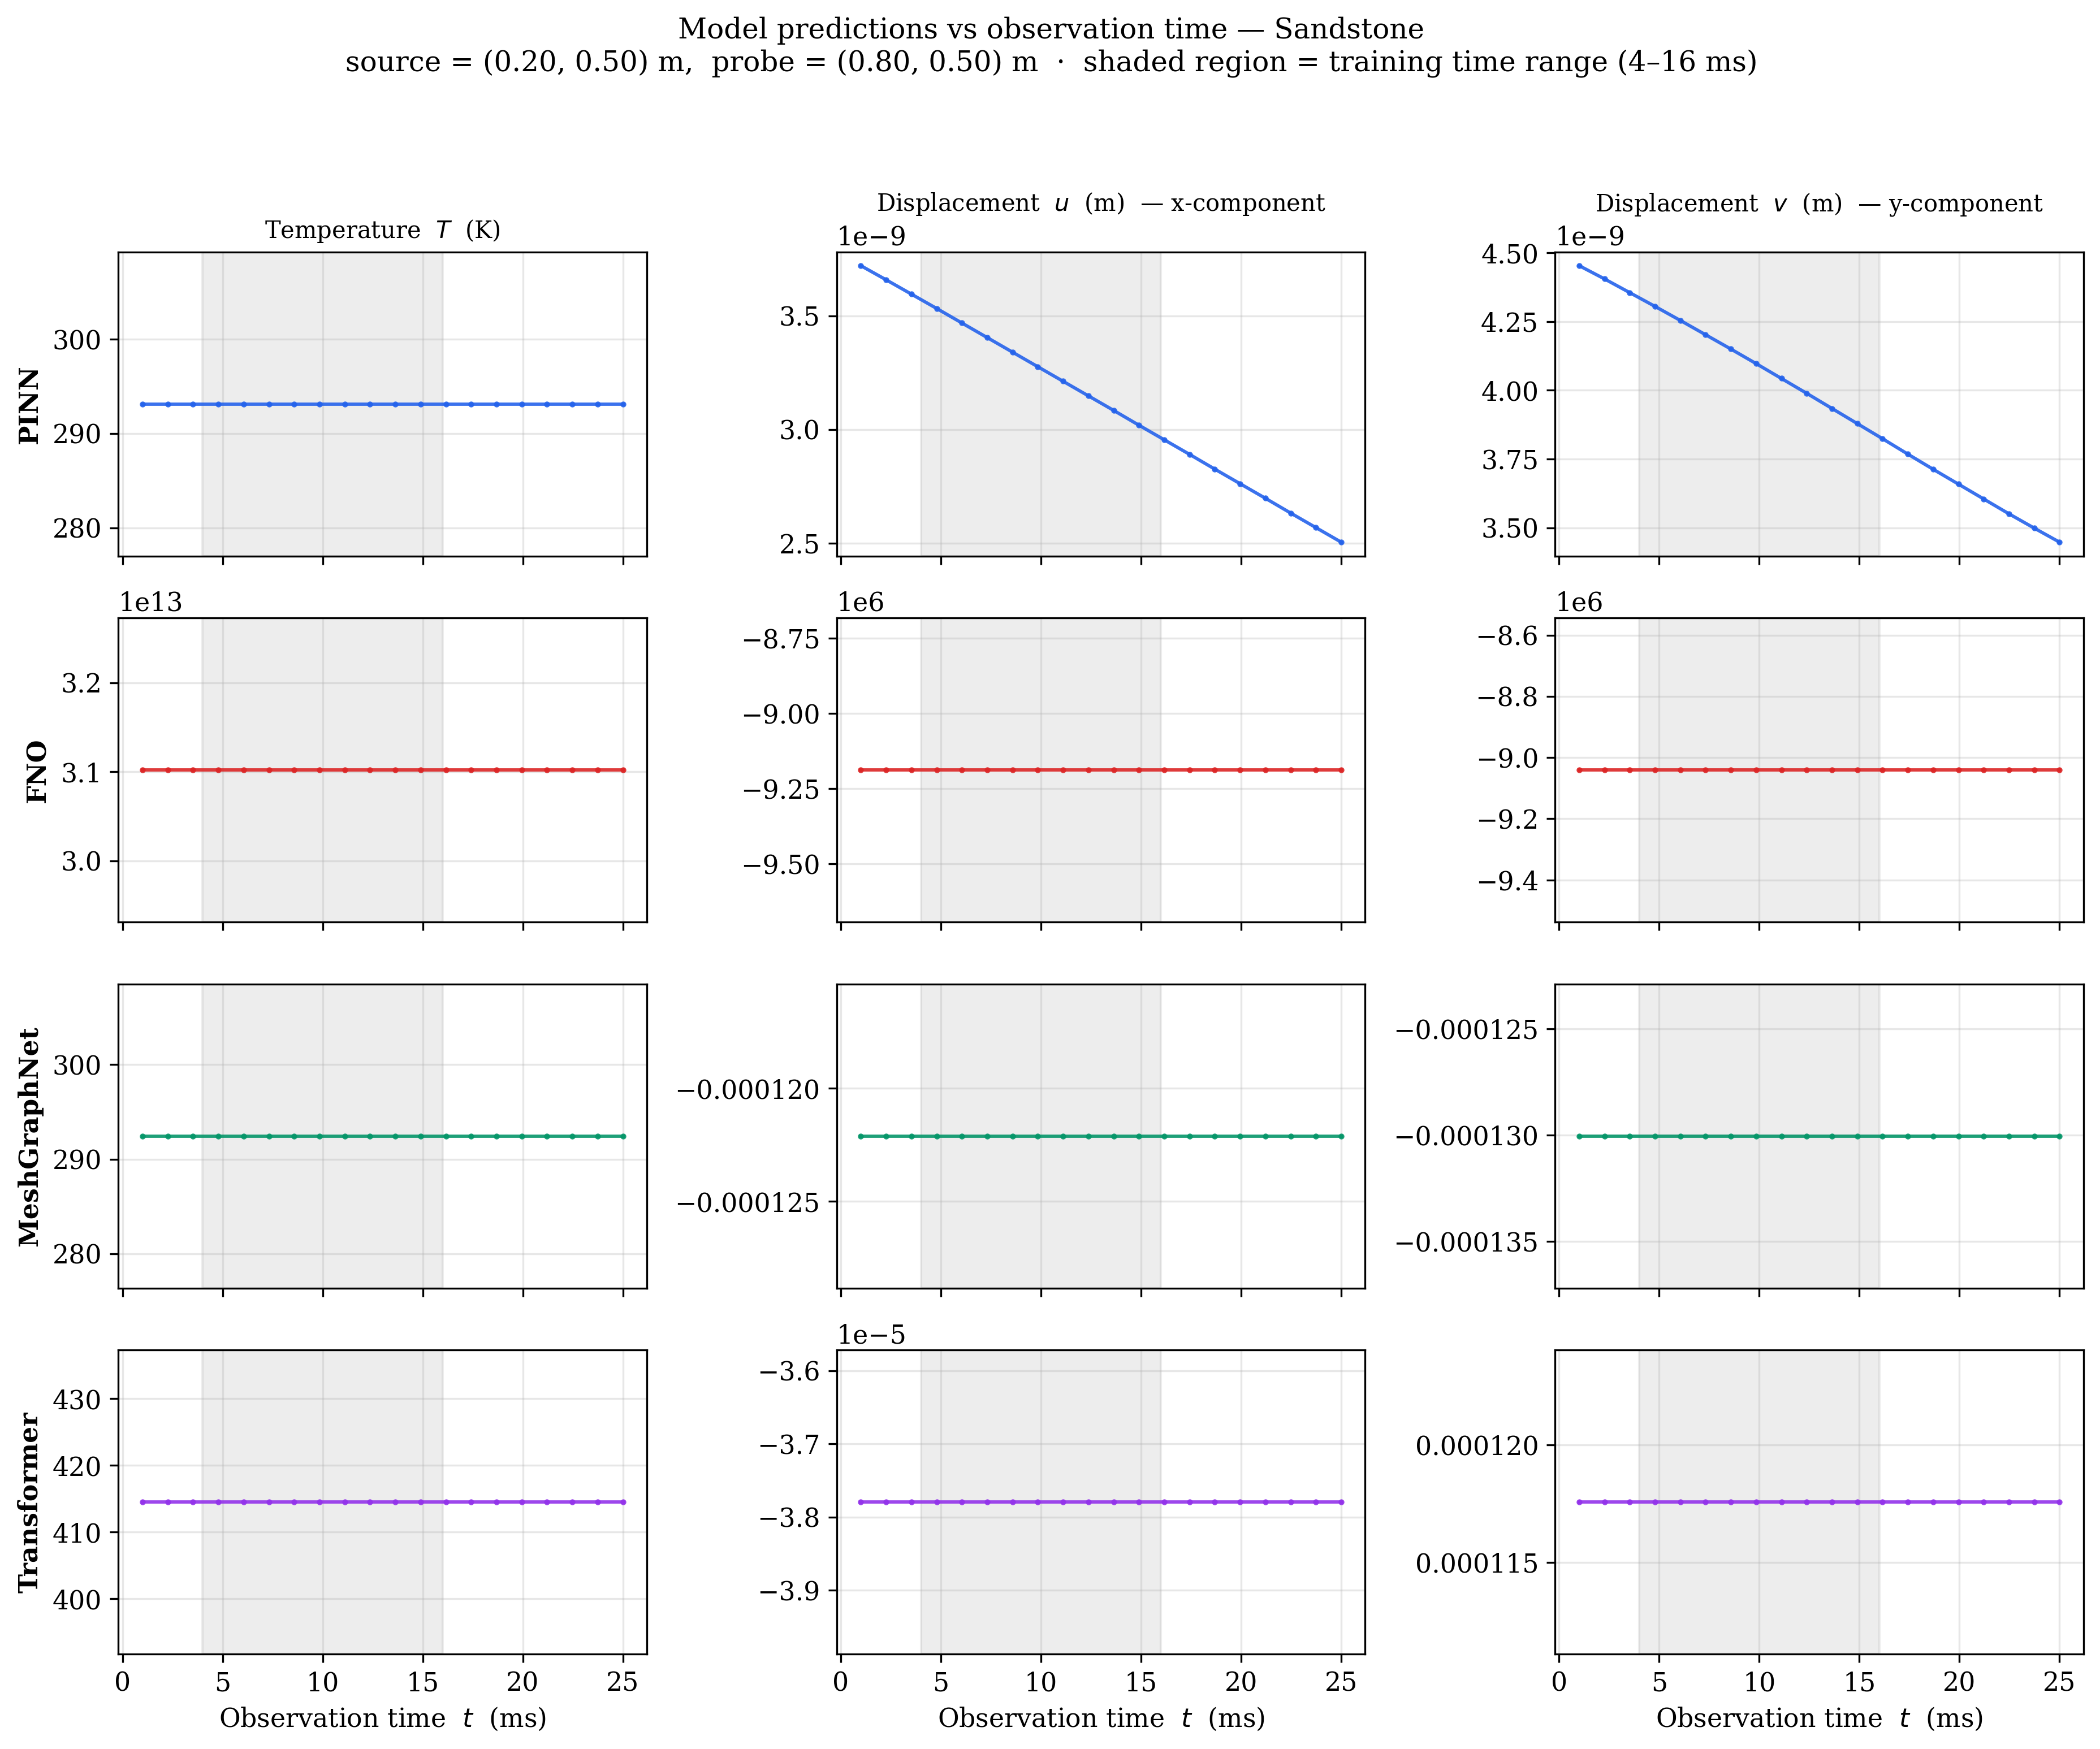
\includegraphics[width=\textwidth]{img/model_timeseries_sandstone}
    \end{column}
    \begin{column}{0.35\textwidth}
      \footnotesize
      \textbf{PINN} is the only route that changes smoothly with the
      requested observation time -- $t$ is a continuous input
      coordinate of the model.
      \vskip 4pt
      \textbf{FNO, MeshGraphNet, Transformer} behave as fixed-horizon
      operators in the current implementation: the probe value remains
      almost unchanged across the tested time range.
      \vskip 4pt
      This is an architectural consequence, not a plotting artefact.
    \end{column}
  \end{columns}
\end{frame}

\begin{frame}{Threats to Validity}
  \begin{enumerate}
    \item \textbf{Limited training data.}
          The COMSOL-derived pilot configuration is not a full
          field-validated geological database; generalisation beyond
          the trained envelope is not yet established.
    \item \textbf{FNO normalisation.}
          The current 2D adaptation has inconsistent output scales for
          several metrics; not a physically reliable route yet.
    \item \textbf{Prototype-level latency.}
          Numbers reflect the development machine, not a production
          deployment.
    \item \textbf{Analytical reference is isotropic.}
          $r/V_{p}$ is useful as a sanity check but is not a substitute
          for a full thermoelastic validation study.
  \end{enumerate}
\end{frame}

% ===========================================
\sectionframe{Section 5 -- Conclusion}
\section{Conclusion}
% ===========================================

\begin{frame}{Summary of Findings}
  \begin{columns}[T]
    \begin{column}{0.33\textwidth}
      \begin{block}{What works}
        \footnotesize
        All four services respond successfully; no fallback responses
        are used. The v2 contract supports a fair end-to-end
        comparison across model families.
      \end{block}
    \end{column}
    \begin{column}{0.33\textwidth}
      \begin{block}{Model behaviour}
        \footnotesize
        PINN: physically stable, only route inside the $10\%$
        accuracy band. MGN: stable but fixed-horizon. Transformer:
        fast and material-sensitive. FNO: integration branch only,
        pending calibration.
      \end{block}
    \end{column}
    \begin{column}{0.33\textwidth}
      \begin{block}{Material effect}
        \footnotesize
        Sandstone is generally slower than basalt across routes.
        Model-family differences still dominate the spread over
        material differences.
      \end{block}
    \end{column}
  \end{columns}
\end{frame}

\begin{frame}{Recommendations and Next Steps}
  \begin{enumerate}
    \item \textbf{Use PINN as the physics-informed baseline} for the
          directional prediction problem in this thesis.
    \item \textbf{Use MeshGraphNet} as the mesh-aware surrogate
          candidate.
    \item \textbf{Use the Transformer route} as the fast
          coordinate-query candidate.
    \item \textbf{Correct FNO output normalisation} and re-run the
          balanced basalt/sandstone/granite/limestone sweep on the
          same pipeline.
    \item \textbf{Add physics-informed residuals} to the Transformer
          route and time-conditioned rollout to MeshGraphNet.
  \end{enumerate}
\end{frame}

% ===========================================
%  CLOSING
% ===========================================

\standoutframe{%
  {\rmfamily\mdseries\LARGE\color{UUblack} Physics-aware surrogates,}\vspace*{-0.2cm}\\
  {\opensans\fontseries{l}\LARGE\itshape\color{UUblack} faster geological prediction.}%
}

\thankframe{Thank you for your attention}{Questions?}

\closingframe

\end{document}
